\documentclass[11pt,a4paper]{article}
\usepackage[french]{babel}
\usepackage[utf8]{inputenc}
\usepackage{mathtools,amssymb,amsthm}
\usepackage{mathrsfs,stmaryrd}
\usepackage{fancybox,mdframed,multicol,comment,enumitem}
\usepackage{microtype}

\usepackage{hyperref}
\hypersetup{
    colorlinks=true,       % false: boxed links; true: colored links
    linkcolor=blue,          % color of internal links
    citecolor=blue,        % color of links to bibliography
    filecolor=blue,      % color of file links
    urlcolor=black           % color of external links
}

%\usepackage[dvipsnames]{xcolor}

\usepackage[normalem]{ulem} % pour souligner avec changements de ligne
\usepackage{pgf,pgfmath,tikz}
\usetikzlibrary{arrows}
\usetikzlibrary[patterns]
\tikzset{every picture/.style={execute at begin picture={
   \shorthandoff{:;!?};}
}}

\newcommand*\circled[1]{\tikz[baseline=(char.base)]{
            \node[shape=circle,draw,inner sep=2pt] (char) {#1};}}


\def\point{node {$\bullet$}}

\usepackage{tkz-euclide}



\theoremstyle{definition}
\newtheorem{theoreme}{Théorème}[section]
\newtheorem{definition}[theoreme]{Définition}
\newtheorem{definitions}[theoreme]{Définitions}
\newtheorem{lemme}[theoreme]{Lemme}
\newtheorem{proposition}[theoreme]{Proposition}
\newtheorem{corollaire}[theoreme]{Corollaire}
\newtheorem{remarque}[theoreme]{Remarque}
\newtheorem{ex}{Problème}

\newcommand{\N}{\mathbb N}
\newcommand{\Z}{\mathbb Z}
\newcommand{\Q}{\mathbb Q}
\newcommand{\R}{\mathbb R}
\newcommand{\C}{\mathbb C}
\newcommand{\U}{\mathbb U}
\newcommand{\F}{\mathbb F}
\newcommand{\G}{\mathbb G}

\newcommand*{\etoile}
{
\begin{center}
$\star$\par
$\star$\hspace*{3ex}$\star$
\end{center}
}

\newcommand{\ensemble}[2]{\left \{ #1  
    \ifx&#2&%
       %
    \else%
       \, \middle | \, #2%
    \fi%
\right \}}

\newcommand{\modulo}[1]{\:\left(\operatorname{mod}\:#1\right)}

% délimiteurs

\DeclarePairedDelimiter{\abs}{\lvert}{\rvert}
\DeclarePairedDelimiter{\ceil}{\lceil}{\rceil}
\DeclarePairedDelimiter{\floor}{\lfloor}{\rfloor}


%%%%%%%%%%%%%%%%%%%%%%%%%%%%%%%%%
%%%%%% MISE EN FORME CLUB %%%%%%%
%%%%%%%%%%%%%%%%%%%%%%%%%%%%%%%%%

\pagestyle{empty}

\usepackage[margin=2.5cm]{geometry}
\everymath{\displaystyle}
\usepackage{fourier}
%\usepackage{fourier,eulervm}% Adobe Utopia et Euler
% En-tête des feuilles :

\newcommand{\enTete}[1]{
\noindent \textbf{\textsf{\href{http://depmath-nancy.univ-lorraine.fr/club/}{Club Mathématique de Nancy} \hfill Institut Élie Cartan}}
\hrule
\begin{center}
{\Huge \textbf{#1}}
\end{center}
\hrule
\vspace{1em}
}

\newcommand{\avertissement}{\begin{mdframed}[linewidth=1pt]\textbf{AVERTISSEMENT ! Ce document est un brouillon qui sert de catalogue pour les feuilles d'exos du club mathématique de Nancy \url{https://dmegy.perso.math.cnrs.fr/club/}. Ne pas diffuser tel quel aux élèves ni de façon large sur le net, il reste des coquilles et énoncés parfois peu précis. Ce document a vocation a rester inachevé. Il peut néanmoins être utile aux enseignants. Enfin, ce document change en permanence, la version à jour est récupérable sur \url{https://github.com/dmegy/clubmath-exos}.}\end{mdframed}}




% - - - - - - - - - - - - - -
% PARAMETRAGE DU PACKAGE ANSWERS 
% POUR LES INDICATIONS ET CORRECTIONS
% - - - - - - - - - - - - - - 

\usepackage{answers}

\Newassociation{sol}{Soln}{solutions}
% ira dans le fichier d'identifiant 'solutions'
% et écrira les solutions dans un environnement 'Soln'
\Newassociation{hint}{Hint}{indications}

\newenvironment{exo}{\begin{ex} \label{enonce.\theex} }{\end{ex} }

\renewenvironment{Soln}[1]{\noindent{\bf Correction de l'exercice \ref{enonce.#1}.} \\ }

\renewenvironment{Hint}[1]{ \noindent{\bf Exercice  \ref{enonce.#1}.} \label{hint.#1}}


% - - - - - - - - - - - - - - 
% FIN PARAMETRAGE ANSWERS
% - - - - - - - - - - - - - - 

%-----------------------------
% MACROS POUR LES FEUILLES DE TD


\newenvironment{feuilleTD}{


\Opensolutionfile{indications}[\jobname_hints]
\Opensolutionfile{solutions}[\jobname_sol]
}{
\Closesolutionfile{indications}
\Closesolutionfile{solutions}
}

\newcommand{\indications}{
\newpage
\noindent {\Large \bf Indications} \hrulefill

\vspace{1em}
\Readsolutionfile{indications}
}

\newcommand{\correction}{
\newpage
\hrule
\begin{center}
{\Large \bf Correction}
\end{center}
\hrule
\vspace{1em}
\Readsolutionfile{solutions}
}



\begin{document}
\Opensolutionfile{indications}[_\jobname_hints]
\Opensolutionfile{solutions}[_\jobname_sol]


\title{Autour du théorème de Pythagore}
\author{Damien Mégy}
\maketitle

Catalogue d'exos sur Pythagore pour le Club Mathématique de Nancy. Rédaction en cours, ne pas diffuser.


(Les exercices sont faisables sans connaître le concept de cosinus ni de sinus, uniquement avec Pythagore.)



\begin{exo}
On considère une ligne brisée $ABCDE$ avec des angles droits et des distances comme sur la figure.
Calculer la distance $AE$.
\begin{center}
\begin{tikzpicture}[rotate=-50]
\tkzDefPoint(0,0){A}
\tkzDefPoint(1,0){B}
\tkzDefPoint(1,2){C}
\tkzDefPoint(4,2){D}
\tkzDefPoint(4,6){E}
\tkzMarkRightAngles[size=.2](A,B,C B,C,D C,D,E)
\tkzDrawSegments[very thick](A,B B,C C,D D,E)
\tkzLabelSegment[below left](A,B){$1$}
\tkzLabelSegment(B,C){$2$}
\tkzLabelSegment(C,D){$3$}
\tkzLabelSegment(D,E){$4$}
\tkzDrawPoints(A,B,C,D,E)
\tkzLabelPoints[left](A)\tkzLabelPoints[below](B)\tkzLabelPoints[above](C)\tkzLabelPoints[below](D)\tkzLabelPoints[right](E)

\end{tikzpicture}
\end{center}
\begin{hint}
Trouver un rectangle dont $[AE]$ est une diagonale et appliquer Pythagore.
\end{hint}
\begin{sol}
Considérons un point $P$ tel que $BCDP$ est un rectangle. Alors $APE$ est rectangle en $P$.
On a alors $AE^2 = (1+3)^2+(2+4)^2=4^2+6^2=52$, d'où $AE=2\sqrt{13}$.
\end{sol}
\end{exo}

Double Pythagore : \url{https://www.youtube.com/watch?v=izbTPRWuO50} (facile)

Un trapèze rectangle, aussi.

\begin{exo}
Dans un demi-cercle de rayon $1$cm, on inscrit un autre demi-cercle plus petit, comme sur la figure.
Quel est le rayon du petit demi-cercle ?
\begin{center}
\begin{tikzpicture}[scale=2]
\tkzDefPoint(0,0){O} \tkzDefPoint(1,0){A}  \tkzDefPoint(-1,0){B}  
\tkzDefPoint(0,1/sqrt{2}){O'} \tkzDefPoint(1/sqrt{2},1/sqrt{2}){C}\tkzDefPoint(-1/sqrt{2},1/sqrt{2}){D}
\tkzDrawSemiCircle[black](O',D)
\tkzDrawSemiCircle[black,very thick](O,A)
\tkzDrawSegment[very thick](A,B)
\tkzDrawSegment(C,D)
\end{tikzpicture}
\end{center}
\end{exo}




\begin{exo}[Le triangle $30^\circ-60^\circ-90^\circ$]
Le triangle $ABC$ a des angles qui mesurent $30^\circ$, $60^\circ$ et $90^\circ$.
Son hypoténuse $AB$ mesure $1$ cm.
Quelle est la longueur des deux autres côtés ?
\begin{center}
\begin{tikzpicture}[scale=2.5]
\tkzDefPoint(0,1){B} \tkzDefPoint(sqrt{3},0){A} \tkzDefPoint(0,0){C}
\tkzDefBarycentricPoint(A=1,B=1,C=1)\tkzGetPoint{G}
\tkzDrawPolygon[very thick](A,B,C)
\tkzMarkRightAngle(A,C,B)
\tkzAutoLabelPoints[center=G](A,B,C)
\tkzLabelSegment[above right](A,B){$1$}
\tkzLabelSegment[below](C,A){?} \tkzLabelSegment[left](B,C){?}
\tkzLabelAngle[pos=.3](C,B,A){$60^\circ$}
\end{tikzpicture}
\end{center}
\begin{hint}
Considérer la symétrie axiale d'axe $(AC)$.
\end{hint}
\begin{sol}
On obtient un triangle équilatéral quand on dédouble le triangle suivant l'axe proposé. On en déduit qu'un côté mesure $1/2$, et ensuite Pythagore donne $\sqrt{1-\frac14} = \frac{\sqrt 3}{2}$ pour le troisième côté.
\end{sol}
\end{exo}



Dans toute la suite, un triangle \og $3-4-5$\fg{} est un triangle dont les côtés mesurent $3$cm, $4$cm et $5$cm. C'est un triangle rectangle, comme on peut le vérifier à l'aide du théorème de Pythagore.





\begin{exo}
% source : chaîne PreMath : https://www.youtube.com/watch?v=_WhmxcPQX4U 
Dans deux demi-cercles identiques, on inscrit d'une part un rectangle $ABCD$ formé de quatre petits carrés juxtaposés, et d'autre part un carré $EFGH$.
Lequel de $ABCD$ et $EFGH$ a la plus grande aire ?

\begin{center}
\begin{tikzpicture}
\tkzDefPoint(-2,1){A} \tkzDefPoint(-2,0){B}
\tkzDefPoint(2,0){C} \tkzDefPoint(2,1){D}
\tkzDrawPolygon(A,B,C,D)
\draw  (-1,0) -- (-1,1);
\draw  (0,0) -- (0,1);
\draw  (1,0) -- (1,1);
\tkzDefPoint(0,0){O}
\tkzDefPoint(-sqrt{5},0){P}
\tkzDefPoint(sqrt{5},0){Q}
\tkzDrawSemiCircle[black, very thick](O,Q)
\tkzDrawSegment(P,Q)
\tkzDrawPoints(A,B,C,D)
\tkzLabelPoints[above left](A) \tkzLabelPoints[below](B) \tkzLabelPoints[below](C) \tkzLabelPoints[above right](D)
\end{tikzpicture}
\hspace{1cm}
\begin{tikzpicture}
\tkzDefPoint(-1,2){E} \tkzDefPoint(-1,0){F}
\tkzDefPoint(1,0){G} \tkzDefPoint(1,2){H}
\tkzDrawPolygon(E,F,G,H)
\tkzDefPoint(0,0){O}
\tkzDefPoint(-sqrt{5},0){P}
\tkzDefPoint(sqrt{5},0){Q}
\tkzDrawSemiCircle[black, very thick](O,Q)
\tkzDrawSegment(P,Q)
\tkzDrawPoints(E,F,G,H)
\tkzLabelPoints[above left](E) \tkzLabelPoints[below](F) \tkzLabelPoints[below](G) \tkzLabelPoints[above right](H)
\end{tikzpicture}
\end{center}
\begin{sol}
En appliquant le théorème de Pythagore, on voit que les deux aires sont égales  à $\dfrac 45 R^2$ !
\end{sol}

\end{exo}






\begin{exo}
On considère deux cercles de rayon $2$cm et $3$cm qui ont un unique point de contact entre eux.
Ils sont tous deux tangents en $P$ et $Q$ à une certaine droite.
Quelle est la distance $PQ$ ?
\begin{center}
\begin{tikzpicture}[scale=.7]
\tkzDefPoint(0,2){O}\tkzDefPoint(sqrt{24},3){O'}
\tkzDefPoint(0,0){P}\tkzDefPoint(sqrt{24},0){Q}
\tkzDrawCircle[black,thick](O,P)
\tkzDrawCircle[black,thick](O',Q)
\tkzDrawLine(P,Q)
\tkzDrawPoints(P,Q)
\tkzLabelPoints(P,Q)
\end{tikzpicture}
\end{center}
\begin{hint}
\end{hint}
\begin{sol}
\end{sol}
\end{exo}


\begin{exo}[Spirale pythagoricienne]
Cette spirale est formée de triangles rectangles juxtaposés. On a 
$OA=AB=BC=CD= DE=EF=FG=GH=HI=1$.
Que vaut $OI$ ?
\begin{center}
%\definecolor{qqwuqq}{rgb}{0.,0.39215686274509803,0.}
\definecolor{qqwuqq}{rgb}{0,0,0}
\begin{tikzpicture}[line cap=round,line join=round,>=triangle 45,rotate=30,scale=1.2]
%\clip(-1.28,-3.08) rectangle (4.72,2.7);
%angles:
\draw[color=qqwuqq,fill=qqwuqq,fill opacity=0.10000000149011612] (0.28284271247461906,0.) -- (0.28284271247461906,0.28284271247461906) -- (0.,0.28284271247461906) -- (0.,0.) -- cycle; 
\draw[color=qqwuqq,fill=qqwuqq,fill opacity=0.10000000149011612] (0.2,0.8) -- (0.4,1.) -- (0.2,1.2) -- (0.,1.) -- cycle; 
\draw[color=qqwuqq,fill=qqwuqq,fill opacity=0.10000000149011612] (0.7549360435341675,1.428337411163077) -- (1.033705413557638,1.476166673510697) -- (0.9858761512100178,1.7549360435341674) -- (0.7071067811865475,1.7071067811865475) -- cycle; 
\draw[color=qqwuqq,fill=qqwuqq,fill opacity=0.10000000149011612] (1.5947420120656104,1.6108727725011909) -- (1.86007799947673,1.5129094437267652) -- (1.9580413282511557,1.7782454311378848) -- (1.692705340840036,1.8762087599123105) -- cycle; 
\draw[color=qqwuqq,fill=qqwuqq,fill opacity=0.10000000149011612] (2.4245267948738216,1.3363429000893319) -- (2.6180399842767828,1.1300599741669628) -- (2.824322910199152,1.3235731635699242) -- (2.6308097207961905,1.5298560894922932) -- cycle; 
\draw[color=qqwuqq,fill=qqwuqq,fill opacity=0.10000000149011612] (3.0476710481598275,0.7080978975204855) -- (3.1401089613180893,0.440786782504769) -- (3.407420076333806,0.5332246956630311) -- (3.314982163175544,0.8005358106787476) -- cycle; 
\draw[color=qqwuqq,fill=qqwuqq,fill opacity=0.10000000149011612] (3.359379289033147,-0.12909847315852738) -- (3.3439260622996714,-0.41151872346562524) -- (3.626346312606769,-0.4269719501991008) -- (3.6417995393402447,-0.1445516998920029) -- cycle; 
\draw[color=qqwuqq,fill=qqwuqq,fill opacity=0.10000000149011612] (3.328447719041178,-1.028752263517281) -- (3.214141911983702,-1.2874686767440788) -- (3.4728583252105,-1.4017744838015544) -- (3.5871641322679757,-1.1430580705747568) -- cycle; 



\draw[thick]  (1.,0.)-- (0.,0.);
\draw[thick]  (0.,1.)-- (1.,0.);
\draw[thick]  (0.,1.)-- (0.,0.);
\draw[thick] (1.,0.)-- (0.7071067811865475,1.7071067811865475);
\draw[thick]  (1.,0.)-- (1.692705340840036,1.8762087599123105);
\draw[thick]  (1.,0.)-- (2.6308097207961905,1.5298560894922932);
\draw[thick]  (1.,0.)-- (3.314982163175544,0.8005358106787476);
\draw[thick]  (1.,0.)-- (3.6417995393402447,-0.1445516998920029);
\draw[thick]  (1.,0.)-- (3.5871641322679757,-1.1430580705747568);
\draw[thick] (3.183032075771265,-2.057758721559405)-- (1.,0.);
\draw[thick]  (0.,1.)-- (0.7071067811865475,1.7071067811865475);
\draw[thick] (0.7071067811865475,1.7071067811865475)-- (1.692705340840036,1.8762087599123105);
\draw[thick]  (1.692705340840036,1.8762087599123105)-- (2.6308097207961905,1.5298560894922932);
\draw[thick] (2.6308097207961905,1.5298560894922932)-- (3.314982163175544,0.8005358106787476);
\draw[thick]  (3.314982163175544,0.8005358106787476)-- (3.6417995393402447,-0.1445516998920029);
\draw[thick] (3.6417995393402447,-0.1445516998920029)-- (3.5871641322679757,-1.1430580705747568);
\draw[thick]  (3.183032075771265,-2.057758721559405)-- (3.5871641322679757,-1.1430580705747568);


\draw[thick]  (0.,0.) node {$\bullet$};
\draw[thick]  (-0.36,0.09) node {$A$};
\draw[thick] (0.,1.) node {$\bullet$};
\draw[thick]  (-0.36,1.37) node {$B$};
\draw[thick] (1.,0.) node {$\bullet$};
\draw[thick]  (0.78,-0.35) node {$O$};
\draw[thick]  (0.7071067811865475,1.7071067811865475) node {$\bullet$};
\draw[thick]  (0.5,2.17) node {$C$};
\draw[thick]  (1.692705340840036,1.8762087599123105) node {$\bullet$};
\draw[thick]  (1.84,2.21) node {$D$};
\draw[thick]  (2.6308097207961905,1.5298560894922932) node {$\bullet$};
\draw[thick]  (2.78,1.85) node {$E$};
\draw[thick]  (3.314982163175544,0.8005358106787476) node {$\bullet$};
\draw[thick]  (3.46,1.13) node {$F$};
\draw[thick]  (3.6417995393402447,-0.1445516998920029) node {$\bullet$};
\draw[thick]  (3.78,0.19) node {$G$};
\draw[thick]  (3.5871641322679757,-1.1430580705747568) node {$\bullet$};
\draw[thick]  (3.88,-1.07) node {$H$};
\draw[thick]  (3.183032075771265,-2.057758721559405) node {$\bullet$};
\draw[thick] (3.54,-2.11) node {$I$};



\end{tikzpicture}
\end{center}
\begin{hint}
Appliquer Pythagore dans les triangles rectangles en partant du plus petit. Le résultat demandé est un nombre entier.
\end{hint}
\begin{sol}
\end{sol}
\end{exo}



% - - - - - - - - - - - - - - - - - - - - 

\begin{exo}% triangles égaux
Dans un carré $ABCD$, on trace un point $M$ sur le côté $[BC]$.
Les perpendiculaires à $(AM)$ passant par $D$ et $B$ coupent $(AM)$ en $P$ et $Q$.
Sachant que $DP=5$cm et $BQ=4$cm, déterminer l'aire du carré $ABCD$.%\\
%(Bonus : calculer ensuite la distance $AM$.)
% a besoin de triangles semblables ou de Thalès.
\begin{center}
\begin{tikzpicture}[rotate=atan(4/5), scale=.8]
\tkzDefPoint(0,0){A} \tkzDefPoint(5,-4){B} \tkzDefPoint(9,1){C} \tkzDefPoint(4,5){D}
\tkzDefBarycentricPoint(A=1,C=1)\tkzGetPoint{G}
\tkzDrawPolygon[very thick](A,B,C,D)
\tkzDefPoint(5+16/5,0){M} \tkzDefPoint(4,0){P}  \tkzDefPoint(5,0){Q}
\tkzDrawSegments(A,M D,P B,Q)
\tkzMarkRightAngle(D,P,A) \tkzMarkRightAngle(B,Q,M)
\tkzDrawPoints(P,Q,M)
\tkzLabelPoints[below left](A) \tkzLabelPoints[below right](B) \tkzLabelPoints[above right](C) \tkzLabelPoints[above left](D)
\tkzLabelPoints[right](M) \tkzLabelPoints[below](P)\tkzLabelPoints[above](Q)
\tkzLabelSegment[below left](D,P){$5$} \tkzLabelSegment[above right](B,Q){$4$} \tkzLabelSegment[left](A,D){?}
\end{tikzpicture}
\end{center}
\begin{hint}
Considérer les triangles $ADP$ et $AQB$
\end{hint}
\begin{sol}
Les triangles $ADP$ et $AQB$ sont égaux : ils ont les mêmes angles et la même hypoténuse.
On en déduit que $AP=4$ et $AQ=5$, et en appliquant le théorème de Pythagore, on trouve le côté du carré : $AB=\sqrt{41}$.
Le carré a donc une aire de $41\mathrm{cm}^2$.

Pour trouver la distance $AM$, il suffit de trouver $QM$. Le plus simple est d'utiliser des triangles semblables, ou Thalès, on trouve $QM=16/5$, donc $AM=5+16/5=41/5$.
\end{sol}
\end{exo}





% - - - - - - - -
\begin{exo}
On considère un triangle isocèle dont les côtés mesurent $13$cm, $13$cm et $10$cm.
Quel est le rayon de son cercle circonscrit ?
\begin{center}
\begin{tikzpicture}[scale=1/3]
\tkzDefPoint(0,0){H}\tkzDefPoint(-5,0){B}\tkzDefPoint(5,0){C}\tkzDefPoint(0,12){A}
\tkzDefCircle[circum](A,B,C) \tkzGetPoint{O} 
\tkzDrawCircle[very thick, black](O,A)
\tkzDrawPolygon(A,B,C)
\tkzLabelSegments[above left](A,B){$13$}\tkzLabelSegments(A,C){$13$}\tkzLabelSegments(B,C){$10$}
\end{tikzpicture}
\end{center}
\begin{hint}
Il y a une hauteur $h$ que l'on peut calculer à l'aide de Pythagore.
Ensuite, si l'on note $H$ le pied de cette hauteur et $O$ le centre du cercle circonscrit, on peut par exemple appliquer Pythagore dans le triangle rectangle $OHB$.
\end{hint}
\begin{sol}
On trouve une hauteur de $12$, et un rayon de $\frac{169}{24}$.
\end{sol}
\end{exo}




\begin{exo}[Zig-Zag dans un carré]
Que vaut  à chaque fois le côté du carré ?
\begin{center}
\begin{tikzpicture}[scale=1,rotate=30]
\draw[very thick] (0,0)  -- (1,0) node[midway, above] {$1$} 
-- (1,2) node[midway, right] {$2$}  
-- (4,2) node[midway, below] {$3$}  ;
\draw[very thick] (0,0) -- (1,3) -- (4,2) -- (3,-1) -- cycle;
\draw [black] (1,0) rectangle (.8,.2) ;
\draw [black] (1,2) rectangle (1.2,1.8) ;
\end{tikzpicture}
\hspace{1cm}
\begin{tikzpicture}[scale=.18,rotate=20]
\draw[very thick] (0,0)  -- (14,0) node[midway, above] {$14$} 
-- (14,7) node[midway, right] {$7$}  
-- (23,7) node[midway, below] {$9$}  ;
\draw[very thick] (0,0) -- (8,15) -- (23,7) -- (15,-8) -- cycle;
\draw [black] (13,0) rectangle (14,1) ;
\draw [black] (14,6) rectangle (15,7) ;
\end{tikzpicture}

\end{center}
\begin{hint}
\end{hint}
\begin{sol}
Le côté vaut $\sqrt{10}$.

Pour le second la source d'origine est : \url{https://twitter.com/0y6tr4/status/1522092641017602049}. Mais en fait le premier est mieux, plus simple
\end{sol}
\end{exo}



% - - - - - - - -
\begin{exo}
Dans un cercle $\mathcal C$, on a une corde $[AB]$ mesurant $4$cm. 
De plus, on sait que la distance entre le milieu de cette corde et le cercle est de $1$cm.
Quel est le rayon du cercle ?
\begin{center}
\begin{tikzpicture}
\tkzDefPoint(-2,0){A} \tkzDefPoint(2,0){B}
\tkzDefPoint(0,0){I} \tkzDefPoint(0,1){P}
\tkzDrawSegment(A,B)
\tkzDrawSegment[dashed](I,P)
\tkzDefPoint(0,-1.5){O}
\tkzDrawCircle[very thick](O,A)
\tkzLabelSegment[below](A,I) {$2$}
\tkzLabelSegment[below](I,B) {$2$}
\tkzLabelSegment[right](I,P) {$1$}
\tkzMarkRightAngle[size=.2](A,I,P)
\tkzDrawPoints(A,B,P)
\tkzLabelPoints[left](A) \tkzLabelPoints[right](B)
\end{tikzpicture}
\end{center}
\begin{hint}
Placer le centre $O$ du cercle. Que vaut la distance de $O$ à la corde, en fonction du rayon $R$ ?
Ensuite, on peut appliquer Pythagore.
\end{hint}
\begin{sol}
Le diamètre vaut $5$cm.
\end{sol}
\end{exo}



% - - - - - -

\begin{exo}
Dans un carré dont les côtés mesurent $1$cm, on inscrit un quart de cercle puis un petit cercle comme sur la figure.
Quel est le rayon du petit cercle ?
\begin{center}
\begin{tikzpicture}[scale=4]
\tkzDefPoint(0,0){O} \tkzDefPoint(1,0){A} \tkzDefPoint(1,1){B} \tkzDefPoint(0,1){C}
\tkzDefPoint(2*sqrt{2}-2,2*sqrt{2}-2){O'}
\tkzDefPoint(1/sqrt{2},1/sqrt{2}){P}
\tkzDrawPoint(O')
\tkzDrawArc[black,thick](O,A)(C)
\tkzDrawPolygon[very thick](O,A,B,C)
\tkzDrawCircle[black,thick](O',P)
\end{tikzpicture}
\end{center}
\begin{hint}
Tracer le centre du petit cercle et décomposer la diagonale du carré en plusieurs segments.
\end{hint}
\begin{sol}
On décompose la diagonale en trois segments : on obtient
\[ \sqrt 2 = 1+R+R\sqrt 2\]
Ceci aboutit à $R=3-2\sqrt{2}$.
\end{sol}
\end{exo}


% - - - - - - - - - - - - - - - - - - - - 


\begin{exo}
Quel est le rayon du cercle inscrit dans un triangle équilatéral de côté $1$cm?
\begin{center}
\begin{tikzpicture}[rotate=-30,scale=1.2]
\tkzDefPoint(0,0){O} \tkzDefPoint(0:2){A}\tkzDefPoint(120:2){B}\tkzDefPoint(240:2){C}
\tkzDefPoint(60:1){P}
\tkzDrawPolygon[very thick](A,B,C)
\tkzDrawCircle(O,P)
\end{tikzpicture}
\end{center}
\begin{hint}
Il est peut-être plus simple de s'imaginer que le cercle est de rayon $1$ et de chercher la taille du triangle équilatéral.
Tracer les hauteurs de ce triangle équilatéral.
\end{hint}
\begin{sol}
On trouve $R=\frac{1}{2\sqrt 3}$. (Si le triangle est de côté $1$.)

Sinon, on peut remarquer que pour un triangle équilatéral, le centre du cercle inscrit est également le centre de gravité, ou le centre du cercle circonscrit. Il se trouve donc au tiers des médianes en partant de la base.
Or, les médianes sont les hauteurs, elles mesurent $\frac{\sqrt 3}{2}$.
\end{sol}
\end{exo}


% - - - - - - -


\begin{exo}
Dans un triangle équilatéral de côté $1$cm, on inscrit un premier cercle, puis trois autres petits cercles, comme sur la figure.
Calculer le rayon $r$ des petits cercles.
\begin{center}
\begin{tikzpicture}[rotate=-30,scale=1.2]
\tkzDefPoint(0,0){O}
\tkzDefPoint(0:2){A}\tkzDefPoint(120:2){B}\tkzDefPoint(240:2){C}
\tkzDefPoint(0:1){P}\tkzDefPoint(120:1){Q}\tkzDefPoint(240:1){R}
\tkzDefPoint(0:4/3){X} \tkzDefPoint(120:4/3){Y} \tkzDefPoint(240:4/3){Z}
\tkzDrawCircle(X,P)
\tkzDrawCircle(Y,Q)
\tkzDrawCircle(Z,R)
\tkzDrawPolygon[very thick](A,B,C)
\tkzDrawCircle(O,P)

\end{tikzpicture}
\end{center}
\begin{hint}
Quelle est la taille des petits cercles, par rapport au grand cercle inscrit ?
\end{hint}
\begin{sol}
Les petits cercles sont trois fois plus petits que le grand cercle, comme on le voit en trançant les tangentes communes aux cercles, ce qui partage le triangle en un hexagone de côté $1/3$ et trois petits triangles équilatéraux.

Comme on sait que $R=\frac{1}{2\sqrt 3}$, on trouve donc $r=\frac{1}{6\sqrt 3}$.
\end{sol}
\end{exo}

% - - - - - - - - - - - - - - - - - - - - 

\begin{exo}
Dans un rectangle de dimensions $3\mathrm{cm}\times 2\mathrm{cm}$, on inscrit deux demi-cercles de même rayon qui se touchent en un seul point, comme sur la figure.
Quel est le rayon de ces deux demi-cercles ? (Ce n'est pas $1$!)
\begin{center}
\begin{tikzpicture}[scale=2]
\draw[very thick] (0,0) rectangle (3,2);
\tkzDefPoint(13/12,0){O} \tkzDefPoint(23/12,2){O'} 
\tkzDefPoint(26/12,0){A} \tkzDefPoint(10/12,2){B} 
\tkzDrawSemiCircle(O,A)
\tkzDrawSemiCircle(O',B)
\tkzDrawPoints(O,O')
\tkzLabelPoints(O,O')
\end{tikzpicture}
\end{center}
\begin{sol}
On peut par exemple projeter le centre du rectangle sur une base, noter $x$ la distance de $O$ à ce projeté, et on obtient alors en considérant la largeur et la hauteur du rectangle :  $3=2R+2x$ et $2=2\sqrt{R^2-x^2}$, c'est-à-dire $1=R^2-x^2=\frac32(R-x)$, d'où finalement le système $R+x=\frac32$ et $R-x=\frac23$ et donc $2R=\frac{9+4}{6}$ et finalement $R=\frac{13}{12}$.

Autre méthode : on projette $O'$ sur la base, et on applique Pythagore dans $OO'H$. On a $OH=3-2R$, donc :
\[ (3-2R)^2+4=4R^2\]
Et donc $13-12R=0$, c'est plus rapide !
\end{sol}
\end{exo}





\begin{exo}[Cercles  tangents]
Les trois petits  cercles sont de rayon $1$.
Le grand cercle leur est simultanément tangent. Quel est son rayon ?
\begin{center}
\begin{tikzpicture}[scale=1]
\draw  (30:{2*sqrt(3)/3}) node {$R=1$}  circle (1);
\draw   (150:{2*sqrt(3)/3}) node {$R=1$} circle (1);
\draw  (270:{2*sqrt(3)/3}) node {$R=1$} circle (1);

\draw[very thick] (0,0) circle ({1+2*sqrt(3)/3});
% rajouter petit cercle ?
\end{tikzpicture}
\end{center}
\begin{hint}
Tracer le triangle (équilatéral) reliant les centres des trois petits cercles. Combien mesure  sa hauteur ?
\end{hint}
\end{exo}




\begin{exo}[Zig-zag dans un cercle]
Quel est le rayon du cercle ci-dessous ?
\begin{center}
\begin{tikzpicture}[scale=.5,rotate=20]
\draw  (0,0) circle ({2*sqrt(5)});
\draw[very thick] (-4,-2) node {$\bullet$}  node[below] {$A$} -- (-4,2) node {$\bullet$} node[left] {$B$} -- (2,2) node {$\bullet$} node[right] {$C$} -- (2,4) node {$\bullet$} node[above] {$D$};
\draw (-4,1.5) -- (-3.5,1.5) --(-3.5,2);
\draw (1.5,2) -- (1.5,2.5) -- (2,2.5);
\draw (-4,0) node[right] {$2$};
\draw (-1,2) node[below] {$3$};
\draw (2,3) node[right] {$1$};
\end{tikzpicture}
\end{center}
\begin{hint}
La droite $(BC)$ recoupe le cercle en  un point $E$. Que dire de $[AE]$ ?
L'objectif est de calculer la distance $CE$, après quoi le rayon du cercle est relativement rapide à obtenir.

Autre indication : il y a une racine carrée dans la réponse.
\end{hint}
\end{exo}

\begin{exo}[Zig-zag dans un cercle,bis]
Quel est le rayon du cercle ci-dessous ?
\begin{center}
\begin{tikzpicture}[scale=1,rotate=20]
\draw  (2.5,0) circle (2.5);
\draw[very thick] (0,0) node {$\bullet$}  node[left] {$A$} 
-- (1,0) node {$\bullet$} node[right] {$B$} node[midway, below] {$1$}
-- (1,2) node {$\bullet$} node[left] {$C$} node[midway, right] {$2$}
-- (4,2) node {$\bullet$} node[above] {$D$} node[midway, below] {$3$};

\draw (1,0) rectangle (.8,.2);
\draw (1,2) rectangle (1.2,1.8);

\end{tikzpicture}
\end{center}
\begin{hint}
La droite $(BC)$ recoupe le cercle en  un point $E$. Que dire de $[AE]$ ?
L'objectif est de calculer la distance $CE$, après quoi le rayon du cercle est relativement rapide à obtenir.
\end{hint}
\begin{sol}
Le diamètre est $5$.
\end{sol}
\end{exo}

\begin{exo}
Quatre carrés placés en damier sont inscrits dans un cercle qu'ils touchent en trois points, comme sur la figure.
Si les carrés mesurent chacun $1\mathrm{cm}^2$, quel est le rayon du cercle ?

\begin{center}
\begin{tikzpicture}[rotate=30]
\fill[color=gray] (0,0) rectangle (1,1);
\fill[color=gray] (1,1) rectangle (2,2);
\fill[color=gray] (1,2) rectangle (0,3);
\fill[color=gray]  (0,3) rectangle (-1,4);
\draw (.5,2.25) circle (sqrt{85}/4);
\draw (0,0) node {$\bullet$};
\draw (1,0) node {$\bullet$};
\draw (-1,4) node {$\bullet$};
\end{tikzpicture}
\end{center}
\begin{hint}
On peut trouver le centre en intersectant les médiatrices de deux cordes.
\end{hint}
\begin{sol}
Le rayon vaut $\sqrt{85}/4$.
\end{sol}
\end{exo}







% - - - - - - - - - - - - - - - - - - - - 

\begin{exo}[Triangle rectangle dans un quart de cercle]
Un triangle rectangle \og $3-4-5$\fg{} est inscrit dans un quart de cercle comme ci-dessous;
Quel est le rayon du quart de cercle ?
\begin{center}
\begin{tikzpicture}[scale=.8]
\draw (0,0) -- ({2*sqrt(5)},0) arc (0:90:{2*sqrt(5)}) -- cycle;
\draw[very thick] (0,{sqrt(5)}) node {$\bullet$} node[left] {$A$}
-- ({2*sqrt(5)},0) node[midway,fill=white] {$5$} node {$\bullet$} node[right] {$B$}
-- ({3*2*sqrt(5)/5},{sqrt(5)+3/sqrt(5)}) node[midway,fill=white] {$4$} node {$\bullet$} node[above] {$C$}
-- cycle node[midway,fill=white] {$3$}  ;
\end{tikzpicture}
\end{center}
% source : https://twitter.com/maliuhudmuaz/status/1315383186852118530 
\begin{hint}
On peut compléter la figure comme suit :
\begin{center}
\begin{tikzpicture}[scale=1]
\draw (0,0) -- ({2*sqrt(5)},0) arc (0:180:{2*sqrt(5)}) node[left] {$D$} node {$\bullet$} -- (0,0) -- (0,{2*sqrt(5)});
\draw[very thick] (0,{sqrt(5)}) node {$\bullet$} node[left] {$A$}
-- ({2*sqrt(5)},0) node[midway,fill=white] {$5$} node {$\bullet$} node[right] {$B$}
-- ({3*2*sqrt(5)/5},{sqrt(5)+3/sqrt(5)}) node[midway,fill=white] {$4$} node {$\bullet$} node[above] {$C$}
-- cycle node[midway,fill=white] {$3$}  ;
%\draw ({-2*sqrt(5)},0)-- (0,{sqrt(5)});
\end{tikzpicture}
\end{center}
Ensuite, on peut prolonger la droite $(AC)$.
\end{hint}
\begin{sol}
Complétons la figure comme suit :
\begin{center}
\begin{tikzpicture}[scale=1]
\draw (0,0) -- ({2*sqrt(5)},0) arc (0:180:{2*sqrt(5)}) node[left] {$D$} node {$\bullet$} -- (0,0) -- (0,{2*sqrt(5)});
\draw[very thick] (0,{sqrt(5)}) node {$\bullet$} node[left] {$A$}
-- ({2*sqrt(5)},0) node[midway,fill=white] {$5$} node {$\bullet$} node[right] {$B$}
-- ({3*2*sqrt(5)/5},{sqrt(5)+3/sqrt(5)}) node[midway,fill=white] {$4$} node {$\bullet$} node[above] {$C$}
-- cycle node[midway,fill=white] {$3$}  ;
\draw ({-2*sqrt(5)},0)-- (0,{sqrt(5)});
\end{tikzpicture}
\end{center}
Comme le triangle $ABC$ est rectangle en $C$, la droite $(AC)$ recoupe le droite $(OB)$ en $D$. Le triangle $DBC$ est rectangle en $C$ et on a $DC=8$ et $BC=4$, donc en appliquant le théorème de Pythagore, on obtient 
\[ DB=\sqrt{64+16}=\sqrt{80} = 4\sqrt5.\]
Le rayon est donc égal à $2\sqrt 5$.
\end{sol}
\end{exo}





%
%\begin{exo}
%\url{https://www.youtube.com/watch?v=og9Ak5ARqe4}
%
%Pas mal mais le rayon que 'on trouve est dégueu... Il faut faire trois fois pythagore.
%\end{exo}










% - - - - - - - - - - - - - - - - - - - - 

\begin{exo}[Le triangle $15^\circ-75^\circ-90^\circ$]
Le triangle $ABC$ a des angles qui mesurent $15^\circ$, $75^\circ$ et $90^\circ$, comme sur la figure ci-dessous. Son hypoténuse $AB$ mesure $1$ cm. 
Montrer que  $AC=\frac{\sqrt 3 +1}{2\sqrt 2}$ puis que $CB=\frac{\sqrt 3 - 1}{2\sqrt 2}$.

% en s'aidant des indications en pointillés sur la figure.

\begin{center}
\begin{tikzpicture}[scale=4]
\tkzDefPoint(-1,0){A}
\tkzDefPoint(0,0){B}
\tkzDefPoint(1,0){D}
\tkzDefPoint({sqrt(3)/2},1/2){E}
\tkzDefPoint({sqrt(3)/2},0){P}
\tkzDefPointBy[projection = onto A--E](B)
\tkzGetPoint{C}
\tkzDrawPolygon[very thick](A,B,C)
%\tkzDrawSegments[dashed](C,E B,E E,D E,P B,D)
%\tkzMarkRightAngles[size=.1](E,P,A A,C,B)
\tkzMarkRightAngles[size=.1](A,C,B)
%\tkzDrawSemiCircle[dashed](B,D)
\tkzLabelPoints[below left](A)
\tkzLabelPoints[below right](B)
\tkzDrawPoint(B)
\tkzLabelPoints[above](C)
\tkzLabelAngle[pos=.4](B,A,C){$15^\circ$}
\tkzLabelSegment[below](A,B){$1$}
\end{tikzpicture}
\end{center}
\begin{hint}
Attention, le calcul peut mener à des expressions qui \emph{semblent} différentes de celles demandées : il faut alors démontrer qu'elles coïncident avec les expressions demandées. Par exemple, on a $\sqrt{6+2\sqrt 5} = 1+\sqrt 5$. (Exercice : pourquoi ?)
\end{hint}
\begin{sol}
Considérer la symétrie axiale d'axe $(AC)$. 
On note $B'$ l'image de $B$ par cette symétrie.
Ensuite, projeter perpendiculairement le point $B$ sur la droite $(AB')$, et reconnaître un triangle rectangle ayant un angle de $30^\circ$ et une hypoténuse de $1cm$.
\end{sol}
\end{exo}



\begin{exo}[Consolidation : le triangle $22,5^\circ-67,5^\circ-90^\circ$]
Le triangle $ABC$ a des angles qui mesurent $22,5^\circ$, $67,5^\circ$ et $90^\circ$, comme sur la figure ci-dessous. Son hypoténuse mesure $1$ cm. 

En utilisant la même technique qu'au problème précédent, calculer $AC$.

\begin{center}
\begin{tikzpicture}[scale=5]
\clip (-1.5,.5) rectangle (.5,-.25);
\tkzDefPoint(-1,0){A}
\tkzDefPoint(0,0){B}
\tkzDefPoint(1,0){D}
\tkzDefPoint({sqrt(2)/2},{sqrt(2)/2}){E}
\tkzDefPoint({sqrt(2)/2},0){P}
\tkzDefPointBy[projection = onto A--E](B)
\tkzGetPoint{C}
\tkzDrawPolygon[very thick](A,B,C)
%\tkzDrawSegments[dashed](C,E B,E E,D E,P B,D)
%\tkzMarkRightAngles[size=.1](E,P,A  A,C,B)
%\tkzDrawSemiCircle[dashed](B,D)
\tkzLabelPoints[below left](A)
\tkzLabelPoints[below right](B)
\tkzDrawPoint(B)
\tkzLabelPoints[above](C)
\tkzLabelAngle[pos=.4](B,A,C){$22,5^\circ$}
\tkzLabelSegment[below](A,B){$1$}
\tkzMarkRightAngle[size=.1](A,C,B)
\end{tikzpicture}
\end{center}
\end{exo}



\begin{exo}
Dans un quart de cercle, on inscrit un demi-cercle comme sur la figure.
Si le rayon du demi-cercle est $1$cm, quel est le rayon du quart de cercle ?
\begin{center}
\begin{tikzpicture}[scale=2,rotate=135]
\tkzDefPoint(0,0){O}\tkzDefPoint(1,0){A} \tkzDefPoint(-1,0){B} 
\tkzDefPoint(1/sqrt{2},1/sqrt{2}){P} \tkzDefPoint(-1/sqrt{2},1/sqrt{2}){Q}
\tkzDrawSemiCircle[black](O,A)
\tkzDefPoint(0,sqrt{2}){O'}
\tkzInterLC(O',Q)(O',A)\tkzGetPoints{Y'}{Y}
\tkzInterLC(O',P)(O',A)\tkzGetPoints{X'}{X}
\tkzDrawArc[black, very thick](O',Y)(X)
\tkzDrawSegments(A,B)
\tkzDrawSegments[very thick](O',X O',Y)
% putain mais qu'est-ce qui m'a pris de faire la figure de cette façon...
\end{tikzpicture}
\end{center}
\begin{sol}
Le rayon du quart de cercle est $\sqrt 3$.
\end{sol}
\end{exo}






% - - - - - - - -
\begin{exo}[Théorème des lunules]
Soit $ABC$ un triangle rectangle en $C$. On trace le demi-cercle de diamètre $[AB]$ qui contient $C$ ainsi que les deux demi-cercles de diamètres $[BC]$ et $[CA]$ extérieurs au triangle. Ces trois demi-cercles délimitent deux lunules, coloriées en noir sur la figure.
Démontrer que la somme des aires de ces deux lunules est exactement égale à l'aire du triangle !
\begin{center}
\begin{tikzpicture}
\begin{scope}[rotate=atan(3/4)]
\draw[line width=1pt,fill=black,color=black] (0,3) arc (90:270:1.5cm) -- cycle;
\draw[line width=1pt,fill=black,color=black]   (0,0) arc (180:360:2cm) -- cycle;
\draw[line width=1pt,fill=white,color=white]  (0,3) arc (180-atan(3/4):360-atan(3/4):2.5cm) -- cycle;
\draw[line width=1pt] (0,0) -- (4,0) node[midway, fill=white] {$b$} -- (0,3) node[midway, fill=white] {$c$}-- cycle node[midway, fill=white] {$a$} ;
\draw (-.3,-.3) node {C};
\draw (4.3,.3) node {A};
\draw (.3,3.3) node {B};
\end{scope}
\end{tikzpicture}
\end{center}
\begin{hint}
Pour calculer l'aire des deux lunules, il faut calculer l'aire du demi-disque de diamètre $[AB]$ et la retrancher à une autre aire.
\end{hint}

\end{exo}


\section{Pythagore et triangles semblables}

\begin{exo}
% triangles semblables, aussi
Dans un triangle rectangle $ABC$ de type \og $3-4-5$\fg, on inscrit un demi-cercle comme sur la figure.
Calculer la distance $AP$.

\begin{center}
\begin{tikzpicture}[scale=1/7]
\tkzDefPoint(0,0){A} \tkzDefPoint(28,0){B} \tkzDefPoint(28,21){C} 
\tkzDefPoint(16-48/5,12-36/5){P}
\tkzDrawPolygon[very thick](A,B,C)
\tkzDefPoint(16,12){O} 
\tkzDrawSemiCircle[black](O,P)
\tkzMarkRightAngle[size=2](C,B,A)
\tkzDrawPoints(A,B,C,P)
\tkzLabelPoints[below left](A) \tkzLabelPoints[below right](B) \tkzLabelPoints[above right](C)
\tkzLabelPoints[above left](P)
\tkzLabelSegment[below](A,B){$4$}
\tkzLabelSegment[right](B,C){$3$}
\end{tikzpicture}
\end{center}
\end{exo}




\begin{exo}[Carrés dans un triangle 3-4-5]
% triangles semblables, aussi
Dans un triangle rectangle $ABC$ de type \og $3-4-5$\fg, on inscrit un carré de deux manières différentes, comme sur les deux figures.
Quelles sont les dimensions des deux carrés ?

\begin{center}
\begin{tikzpicture}[scale=1/7]
\tkzDefPoint(0,0){A} \tkzDefPoint(28,0){B} \tkzDefPoint(28,21){C} 
\tkzDrawPolygon[very thick](A,B,C)
\tkzDefPoint(16,12){O} \tkzDefPoint(16,0){P}  \tkzDefPoint(28,12){Q} 
\tkzDrawSegments(P,O O,Q)
\tkzMarkRightAngle[size=2](C,B,A)
\tkzLabelPoints[below left](A) \tkzLabelPoints[below right](B) \tkzLabelPoints[above right](C)
\end{tikzpicture}
\hspace{1cm}
\begin{tikzpicture}[scale=1/37]
\tkzDefPoint(0,0){A} \tkzDefPoint(148,0){B} \tkzDefPoint(148,111){C} 
\tkzDefPoint(100,0){P} \tkzDefPoint(148,36){Q}
\tkzDefSquare(P,Q)\tkzGetPoints{R}{S}
\tkzDrawPolygon(P,Q,R,S)
\tkzDrawPolygon[very thick](A,B,C)
\tkzMarkRightAngle[size=10](C,B,A)

\tkzLabelPoints[below left](A) \tkzLabelPoints[below right](B) \tkzLabelPoints[above right](C)
\end{tikzpicture}
\end{center}
\begin{sol}
Pour le deuxième carré, on a intérêt à noter $60x$ le côté du carré, de cette façon c'est divisible par $3$, $4$ et $5$. Ensuite on utilise les triangles semblables, mais du coup cet exo est faisable sans Pythagore. On trouve que $x=\frac{1}{37}$ par proportionnalité, le deuxième carré fait donc $60/37$ de côté.

Avec Pythagore ça doit être plus pénible...

Le première carré fait $12/7$ de côté. Là aussi, on a intérêt à noter $12y$ le côté, comme ça c'est divisible par trois et quatre. Et là aussi il vaut mieux faire ça avec des triangles semblables.
Il est plus gros que le premier car $444=12\times 37 \geq 7\times 60=420$. Sur le dessin ça se voir quand même assez nettement.
\end{sol}
\end{exo}






%
%\begin{exo}[]\url{https://twitter.com/archimedes_000/status/1524521121827151874} très bon
%\begin{center}
%\begin{tikzpicture}[scale=1]
%\end{tikzpicture}
%\end{center}
%\begin{hint}
%\end{hint}
%\end{exo}


\begin{exo}[Théorème de la hauteur relative à l'hypoténuse]
Soit $ABC$ un triangle rectangle en $C$ et $H$ le pied de la hauteur issue de $C$.
Montrer que 
\[ HA\times HB = HC^2.\]
\begin{center}
\begin{tikzpicture}[scale=.3]
\draw[very thick] (12,6) -- (15,0) -- (0,0) -- cycle;
\draw[dashed,thick] (12,0) -- (12,6);
\draw (0,0) node {$\bullet$} node[left] {A};
\draw (12,6) node {$\bullet$} node[above] {C};
\draw (15,0) node {$\bullet$} node[right] {B};
\draw (12,0) node {$\bullet$} node[below] {H};
\end{tikzpicture}
\end{center}
\begin{sol}
On fait Pythagore dans les trois triangles et ça se simplifie.

Évidemment on pourrait faire ça plus joliment avec des triangles semblables.
\end{sol}
\end{exo}





\begin{exo}
Dans un triangle rectangle en $A$, en notant $H$ le pied de la hauteur issue de $A$, on a $AB=15$ et $HC=16$.
Calculer $BH$, $AH$ et $AC$.
\begin{center}
\begin{tikzpicture}[scale=1/4]
\tkzDefPoint(0,0){H} \tkzDefPoint(0,12){A} \tkzDefPoint(-9,0){B} \tkzDefPoint(16,0){C}
\tkzDrawPolygon[very thick](A,B,C)
\tkzDrawSegment[dashed](A,H)
\tkzLabelPoints[above](A) \tkzLabelPoints[left](B) \tkzLabelPoints[right](C) \tkzLabelPoints[below](H)
\tkzDrawPoint(H)
\tkzMarkRightAngle[size=1](A,H,B) \tkzMarkRightAngle[size=1](B,A,C)
\tkzLabelSegment[above left](A,B){$15$} \tkzLabelSegment(H,C){$16$} 
\end{tikzpicture}
\end{center}
\begin{sol}
En calculant l'aire du triangle de deux façons, on a $AH\times BC = AB\times AC$.

Ensuite, on peut procéder de plusieurs façons, juste avec Pythagore dans les trois triangles rectangles, ou en remarquant des triangles semblables.
Par exemple, comme $ABH$ et $CAH$ sont semblables, on a, par proportionnalité, le produit en croix $AH^2=HB\times HC = 16 HB$.

Ensuite, en appliquant le théorème de Pythagore dans le triangle $ABH$ rectangle en $H$, on obtient:
\[ 15^2 = AH^2+BH^2 = 16BH+BH^2 = (BH+8)^2-64\]
On en tire $BH+8=\sqrt{15^2+8^2}=\sqrt{289}=17$, d'où $BH=17-8=9$.

Ensuite, on continue et on trouve normalement $AH=12$ et $AC=20$.
\end{sol}
\end{exo}






\begin{exo}[Théorème des cordes sécantes dans un cas particulier]
Dans un cercle, on trace une corde $[AB]$, de milieu $M$. Sa médiatrice intersecte le cercle en $C$ et $D$.
Montrer que
\[ MA\times MB = MC\times MD.\]
\begin{center}
\begin{tikzpicture}[rotate=50,scale=.8]
\tkzDefPoint(-2,0){A} \tkzDefPoint(2,0){B}
\tkzDefPoint(0,1){C} \tkzDefPoint(0,-4){D}
 \tkzDefPoint(0,0){M} 
\tkzDrawSegment(A,B)
\tkzDrawSegment(C,D)
\tkzDefPoint(0,-1.5){O}
\tkzDrawCircle[very thick](O,A)
\tkzMarkRightAngle[size=.2](A,M,C)
\tkzDrawPoints(A,B,C,D,M)
\tkzLabelPoints[left](A) \tkzLabelPoints[right](B)\tkzLabelPoints[left](C) \tkzLabelPoints[right](D)\tkzLabelPoints[above](M)
\tkzMarkSegment[mark=||](A,M)
\tkzMarkSegment[mark=||](M,B)
\end{tikzpicture}
\end{center}
(Note : en réalité, ce théorème reste vrai pour deux cordes \emph{quelconques} s'intersectant en $M$, mais la démonstration est plus difficile et utilise le théorème de l'angle inscrit. La quantité $MA\times MB$ est alors appelée la \emph{puissance} du point $M$ par rapport au cercle.)
\end{exo}









\begin{exo}
Sur un demi-cercle de diamètre $[AC]$, on place un point $M$ de sorte à avoir les longueurs $HB=3$ et $HM=6$. Quel est le rayon du demi-cercle ?
\begin{center}
\begin{tikzpicture}[scale=.3]
\draw[thick] (15,0) -- (0,0) ;
\draw[thick] (12,0) -- (12,6);
\draw[thick] (11,0) -- (11,1) -- (12,1);
\draw[thick] (15,0) arc (0:180:7.5cm);
\draw (13.5,0) node[above] {$3$} ;
\draw (12,3) node[left] {$6$} ;
\draw (0,0) node {$\bullet$} node[left] {A};
\draw (12,0) node {$\bullet$} node[below] {H};
\draw (15,0) node {$\bullet$} node[right] {B};
\draw (12,6) node {$\bullet$} node[below] {M};
\end{tikzpicture}
\end{center}
\begin{sol}
Source : \url{https://twitter.com/Math_World_/status/1519662926860365824}

On peut utiliser le théorème de la hauteur relative à l'hypoténuse (citer référence du problème).

On peut aussi refaire trois fois Pythagore, (ou bien utiliser les triangles semblables, ou utiliser la puissance du point $K$ par rapport au cercle.)
\end{sol}
\end{exo}







\subsection{Calculs avec les racines carrées}

\begin{exo}[Comparaisons de racines carrées]

On considère les trois nombres suivants : $A=3+\sqrt 2$, $B=\sqrt 5 +\sqrt 6$ et $C=1+\sqrt 10$ ?
Classer ces trois nombres du plus petit au plus grand, sans utiliser évidemment de calculatrice.
\begin{hint}
Élever les trois quantités au carré.
\end{hint}
\begin{sol}
On a 
\[
A^2 = 11+6\sqrt 2 = 11+\sqrt{72},\quad
B^2 = 11+2\sqrt{30}=11+\sqrt{120} \quad\text{et}
C^2 = 11+2\sqrt{10}=11+\sqrt{40}.\]
On en déduit que 
\[ C< A < B.\]
\end{sol}
\end{exo}





%Rajouter \url{https://twitter.com/maliuhudmuaz/status/1315383186852118530} utilse les demi-cercles.

\subsection{Circle Packing}

\begin{exo}[circle packing, 1]
Les trois cercles ci-dessous sont tangents et inscrits dans un rectangle. Leurs diamètres valent $3$, $4$ et $6$.
Calculer la longueur $AB$.
\begin{center}
\begin{tikzpicture}[scale=.5]
\draw[very thick] (-1.5,0) rectangle ({3+3*sqrt(6)},6);
\draw  (0,1.5) circle (1.5);
\draw ({3*sqrt(6)},3) circle (3);
\draw ({sqrt(6)},4) circle (2);
\draw (0,0) node {$\bullet$} node[below] {$A$};
\draw ({3*sqrt(6)},0) node {$\bullet$} node[below] {$B$};
\end{tikzpicture}
\end{center}
\begin{hint}
\end{hint}
\begin{sol}
On obtient $AB=\sqrt 6 + 2\sqrt 6 = 3\sqrt 6$. (on fait deux fois Pythagore)
\url{https://twitter.com/0y6tr4/status/1521866673493618690} 
\end{sol}
\end{exo}



\begin{exo}[Cercles dans un carré ]
La figure suivante représente des cercles qui ont  un rayon égal à $1$ et placés dans un carré.
Quelles sont les dimensions des carrés ?
\begin{center}

\begin{tikzpicture}[scale=1]
\draw[thick] ({1/sqrt(2)},{1/sqrt(2)}) circle (1.cm);
\draw[thick] ({-1/sqrt(2)},{-1/sqrt(2)}) circle (1.cm);
\draw [very thick] ({-1-sqrt(2)/2},{-1-sqrt(2)/2}) rectangle ({1+sqrt(2)/2},{1+sqrt(2)/2});
\end{tikzpicture}
\begin{tikzpicture}[line cap=round,line join=round,>=triangle 45,scale=1]
\draw[thick] (1.,1.) circle (1.cm);
\draw [thick] (1.517638090205042,2.931851652578137) circle (1.cm);
\draw [thick] (2.931851652578137,1.5176380902050417) circle (1.cm);
\draw [very thick] (0.,0.)-- (3.932,0.) -- (3.932,3.932)-- (0,3.932) -- cycle;
\end{tikzpicture}
\end{center}
\begin{hint}

\end{hint}
\begin{sol}
\url{https://erich-friedman.github.io/packing/cirinsqu/}
VERIFIER Le carré est de côté $2+\frac{1}{\sqrt 2} + \frac{\sqrt 6}{2}$.

Pour le premier le côté vaut $2+\sqrt2$.
\end{sol}
\end{exo}


\begin{exo}[Cercles dans un carré, bis ]
La figure suivante représente des cercles qui ont  un rayon égal à $1$ et placés dans un carré.
Quelles sont les dimensions du carré ?
\begin{center}

\begin{tikzpicture}[scale=1]
\draw[thick] (0,0) circle (1.cm);
\draw[thick] (0,{8/sqrt(13)}) circle (1.cm);

\draw[thick] ({-6/sqrt(13)},{4/sqrt(13)}) circle (1.cm);
\draw[thick] ({-6/sqrt(13)},{-4/sqrt(13)}) circle (1.cm);
\draw[thick] ({6/sqrt(13)},{4/sqrt(13)}) circle (1.cm);
\draw[thick] ({6/sqrt(13)},{-4/sqrt(13)}) circle (1.cm);
\draw [very thick] ({-6/sqrt(13)-1},{-4/sqrt(13)-1}) rectangle ({6/sqrt(13)+1},{8/sqrt(13)+1}) ;
\end{tikzpicture}

\end{center}
Note : il s'agit du plus petit carré qui peut contenir six disques de rayon un. Ce résultat a été prouvé par Graham en 1963.
\begin{hint}

\end{hint}
\begin{sol}
Le carré a un côté de $2+\frac{12}{\sqrt 13}$. Voir la vidéo \url{https://www.youtube.com/watch?v=ONs1u3xRzrM&t=12s} et bien sûr le site \url{https://erich-friedman.github.io/packing/cirinsqu/}.
\end{sol}
\end{exo}



\subsection{Square packing}




\begin{exo}[Cinq carrés dans un carré]
Les cinq carrés gris sont de côté $1$ et le carré oblique est   incliné de $45^\circ$.
 Quelle est la taille du grand carré ?

\begin{center}
\begin{tikzpicture}[scale=1]
\draw[fill=gray] ({sqrt(2)/4},{sqrt(2)/4}) rectangle ({1+sqrt(2)/4},{1+sqrt(2)/4});
\draw[fill=gray] ({-sqrt(2)/4},{sqrt(2)/4}) rectangle ({-1-sqrt(2)/4},{1+sqrt(2)/4});
\draw[fill=gray] ({sqrt(2)/4},{-sqrt(2)/4}) rectangle ({1+sqrt(2)/4},{-1-sqrt(2)/4});
\draw[fill=gray] ({-sqrt(2)/4},{-sqrt(2)/4}) rectangle ({-1-sqrt(2)/4},{-1-sqrt(2)/4});
\draw[fill=gray] ({-sqrt(2)/2},0)  -- (0,{sqrt(2)/2}) -- ({sqrt(2)/2},0) -- (0,{-sqrt(2)/2}) -- cycle;
\draw[very thick] ({-1-sqrt(2)/4},{-1-sqrt(2)/4}) rectangle ({1+sqrt(2)/4},{1+sqrt(2)/4});
\end{tikzpicture}
\end{center}
Note : Frits Göbel a prouvé en 1979 qu'il s'agit là du plus petit carré pouvant contenir cinq carrés de côté $1$. 

\begin{hint}
\end{hint}
\begin{sol}
\url{https://erich-friedman.github.io/packing/squinsqu/}
\end{sol}
\end{exo}


\begin{exo}[Dix carrés dans un carré]
Pour dix petits carrés, le plus petit carré est le suivant, mais ça n'a été démontré qu'en 2003 par Walter Stromquist. Quelle est la taille du carré ? (Les carrés obliques sont toujours  inclinés de $45^\circ$.)
\begin{center}
\begin{tikzpicture}[scale=1]

%\draw[fill=gray] ({sqrt(2)/4},{sqrt(2)/4}) rectangle ({1+sqrt(2)/4},{1+sqrt(2)/4});
\draw[fill=gray] ({-sqrt(2)/4},{sqrt(2)/4}) rectangle ({-1-sqrt(2)/4},{1+sqrt(2)/4});
\draw[fill=gray] ({sqrt(2)/4},{-sqrt(2)/4}) rectangle ({1+sqrt(2)/4},{-1-sqrt(2)/4});
\draw[fill=gray] ({-sqrt(2)/4},{-sqrt(2)/4}) rectangle ({-1-sqrt(2)/4},{-1-sqrt(2)/4});

\draw[fill=gray] ({-sqrt(2)/4},{1+sqrt(2)/4}) rectangle ({-1-sqrt(2)/4},{2+sqrt(2)/4});
\draw[fill=gray] ({1-sqrt(2)/4},{1+sqrt(2)/4}) rectangle ({-sqrt(2)/4},{2+sqrt(2)/4});

\draw[fill=gray] ({1+sqrt(2)/4},{-sqrt(2)/4}) rectangle ({2+sqrt(2)/4},{-1-sqrt(2)/4});
\draw[fill=gray] ({1+sqrt(2)/4},{1-sqrt(2)/4}) rectangle ({2+sqrt(2)/4},{-sqrt(2)/4});

\draw[fill=gray] ({1+sqrt(2)/4},{1+sqrt(2)/4}) rectangle ({2+sqrt(2)/4},{2+sqrt(2)/4});

\draw[fill=gray] ({-sqrt(2)/2},0)  -- (0,{sqrt(2)/2}) -- ({sqrt(2)/2},0) -- (0,{-sqrt(2)/2}) -- cycle;
\draw[fill=gray]  (0,{sqrt(2)/2}) -- ({sqrt(2)/2},0) -- ({sqrt(2)},{sqrt(2)/2}) -- ({sqrt(2)/2},{sqrt(2)})  --cycle;

\draw[very thick] ({-1-sqrt(2)/4},{-1-sqrt(2)/4}) rectangle ({2+sqrt(2)/4},{2+sqrt(2)/4});
\end{tikzpicture}
\end{center}
Ces problèmes pourraient sembler évidents mais ne le sont pas. Par exemple, pour $11$ et $17$ carrés, les meilleures configurations connues à ce jour sont celles ci-dessous mais on ignore encore si elles sont optimales.
\begin{center}
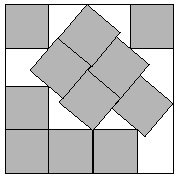
\includegraphics[scale=.5]{sqinsq/s11.png}
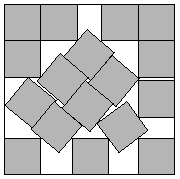
\includegraphics[scale=.5]{sqinsq/s17.png}
\end{center}
\begin{hint}
\end{hint}
\begin{sol}
\url{https://erich-friedman.github.io/packing/squinsqu/}
\end{sol}
\end{exo}


\paragraph{Carrés dans un triangle équilatéral }

\url{https://erich-friedman.github.io/packing/squintri/}

Mettre les premiers, regarder la biblio pour voir si c'est optimal ou pas.

\subsection{AUtre}








%\begin{exo}[]\url{https://twitter.com/archimedes_000/status/1524521121827151874} très bon
%\begin{center}
%\begin{tikzpicture}[scale=1]
%\end{tikzpicture}
%\end{center}
%\begin{hint}
%\end{hint}
%\end{exo}


\begin{exo}[Comparaisons de racines carrées]

On considère les trois nombres suivants : $A=3+\sqrt 2$, $B=\sqrt 5 +\sqrt 6$ et $C=1+\sqrt 10$ ?
Classer ces trois nombres du plus petit au plus grand, sans utiliser évidemment de calculatrice.
\begin{hint}
Élever les trois quantités au carré.
\end{hint}
\begin{sol}
On a 
\[
A^2 = 11+6\sqrt 2 = 11+\sqrt{72},\quad
B^2 = 11+2\sqrt{30}=11+\sqrt{120} \quad\text{et}
C^2 = 11+2\sqrt{10}=11+\sqrt{40}.\]
On en déduit que 
\[ C< A < B.\]
\end{sol}
\end{exo}


\begin{exo}[Vers le théorème de Descartes]
Les trois grands  cercles sont de rayon $1$ et $2$.
Le petit cercle leur est simultanément tangent. Quel est son rayon ?
\begin{center}
\begin{tikzpicture}[rotate=90,scale=1.1]
\draw (-1,0) node {$R=1$}  circle (1);
\draw (1,0) node {$R=1$}  circle (1);
\draw (0,{2*sqrt(2)}) node {$R=2$}  circle (2);
\begin{scriptsize}
\draw[very thick] (0,{2*sqrt(2)-2-(32*sqrt(2)-40)/(28)}) node {$?$} circle ({(32*sqrt(2)-40)/(28)});
\end{scriptsize}
\end{tikzpicture}
\end{center}
\begin{hint}
Tracer les centres des cercles et les relier.
\end{hint}
\end{exo}

%- - - - - - - - - -

\begin{exo}[Cercles de Ford]
Sur une droite graduée, on \og pose\fg{} des cercles de diamètre $\frac{1}{n^2}$ sur les abscisses $\frac{1}{n}$, comme sur la figure ci-dessous. Montrer que tous ces cercles sont tangents, et qu'ils sont tous tangents au cercle de diamètre $1$ posé en l'origine !!
\begin{center}
\begin{tikzpicture}[scale=9]
\clip (-.15,-.1) rectangle (.7,.4);
\draw[very thick] (-0.2,0) -- (.6,0);
\draw (0,0) node[below] {$0$};

\foreach \i in {2, 3, 4, 5, 6, 7}
{
\draw  ({1/\i},{1/(2*\i*\i)}) circle ({1/(2*\i*\i)});
\draw ({1/\i},0) node {$\bullet$} node[below] {$\frac{1}{\i}$};
}

\draw[dashed] (0,1/2) circle (1/2);
\draw (0,0) node {$\bullet$};
\end{tikzpicture}
\end{center}
\begin{hint}
Commencer par montrer que les deux premiers cercles, de diamètres $1/4$ et $1/9$, sont tangents. Dessiner leurs centres.
\end{hint}
\end{exo}

\begin{exo}
blabla
\begin{center}
\begin{tikzpicture}
\end{tikzpicture}
\end{center}
\end{exo}


\begin{exo}
blabla
\begin{center}
\begin{tikzpicture}
\end{tikzpicture}
\end{center}
\end{exo}


\begin{exo}
Identité du parallélogramme
\begin{center}
\begin{tikzpicture}
\end{tikzpicture}
\end{center}
\end{exo}

\begin{exo}
Théorème de la médiane (idem que plus haut)
\url{https://www.youtube.com/watch?v=pqHpU84ggpY}
et chercher variantes sur wikipedia
\begin{center}
\begin{tikzpicture}
\end{tikzpicture}
\end{center}
\end{exo}

\begin{exo}
Plus dur : \url{https://www.youtube.com/watch?v=HbPQco5PVuU}
Demi-cercle avec trois cercles inscrits.
\begin{center}
\begin{tikzpicture}
\end{tikzpicture}
\end{center}
\end{exo}


Plus difficile, avec trinôme et factoriastion : 
\url{https://www.youtube.com/watch?v=KKzf3vh7-pY}



\Closesolutionfile{indications}
\Closesolutionfile{solutions}

\indications
\correction

\end{document}

